\section{Analiza istniejących rozwiązań}
\label{sec:analiza}

\subsection{Zakres i metoda analizy}

Przeanalizowano trzy rozwiązania, z~których każde odpowiada na część problemu
opisanego w~sekcji~\ref{sec:problem}: płatną aplikację mobilną Vademecum
Środków Ochrony Roślin, oficjalną wyszukiwarkę Ministerstwa Rolnictwa
i~Rozwoju Wsi oraz międzynarodową aplikację AgroBase.
Wybrano narzędzia, po które realnie sięgają
użytkownicy projektowanego systemu, gdy muszą dobrać środek ochrony roślin
lub sprawdzić jego dawkowanie.

Każde rozwiązanie opisano według tego samego schematu: opis rozwiązania,
mocne strony, słabe strony oraz wnioski dla projektowanego systemu.

Aplikację Vademecum testowano na telefonie Samsung Galaxy S25 Ultra
(system Android). Dane wyszukiwarki ministerstwa
pobrano i~przeanalizowano 12~października 2026~r. Aplikację AgroBase
testowano w~wersji przeglądarkowej 13~października 2026~r.

\subsection{Vademecum Środków Ochrony Roślin}

\subsubsection{Opis rozwiązania}

Vademecum Środków Ochrony Roślin to aplikacja mobilna na system Android,
pełniąca rolę wyszukiwarki środków ochrony roślin zarejestrowanych w~Polsce.
Pozwala wyszukiwać środki po nazwie, uprawie, agrofagu lub substancji
czynnej, a~dla wybranego środka pokazuje m.in. dawki zarejestrowane dla
poszczególnych upraw, terminy prawne oraz etykietę rejestracyjną. Aplikacja
posiada rekomendację Instytutu Ochrony Roślin -- PIB oraz wyróżnienie FARMER
z~2019~r.

Z~aplikacji można korzystać bez ograniczeń przez 14-dniowy okres próbny.
Później wymagana jest licencja roczna (119~zł, przy automatycznym
odnowieniu 139~zł) lub wieczysta (829~zł).

\subsubsection{Mocne strony}

\begin{itemize}
    \item \textbf{Cztery punkty wejścia do wyszukiwania.}
    Ekran główny prowadzi jednym dotknięciem do wyszukiwania po środku,
    agrofagu, uprawie lub substancji czynnej, dzięki czemu użytkownik
    zaczyna od tego, co w~danej chwili wie.

    \item \textbf{Terminy prawne na karcie środka.}
    Karta środka pokazuje termin ważności pozwolenia, datę końca handlu
    i~okres na zużycie zapasów, więc użytkownik od razu widzi, czy środek
    posiadany w~magazynie wolno jeszcze stosować.

    \item \textbf{Wiarygodność danych.}
    Rekomendacja Instytutu Ochrony Roślin -- PIB wskazuje, że dane zostały
    zweryfikowane przez instytucję naukową.
\end{itemize}

\subsubsection{Słabe strony}

\begin{itemize}
    \item \textbf{Dostępność tylko na Androidzie.}
    Aplikacja nie ma wersji na iOS ani wersji przeglądarkowej. Użytkownik
    telefonu z~innym systemem nie może z~niej skorzystać, a~rolnik lub
    doradca nie sprawdzi informacji na komputerze stacjonarnym czy laptopie,
    na którym przeglądanie danych mogłoby być wygodniejsze.

    \item \textbf{Ekran główny i~licencja.}
    Ekran główny zawiera cztery przyciski prowadzące do wyszukiwarek oraz
    informację o~rodzaju licencji. Podczas testów nie znaleziono możliwości
    wykupienia licencji z~poziomu aplikacji przed upływem 14-dniowego okresu
    próbnego -- komunikat odsyła do sklepu Google Play. Aplikacja nie
    uwzględnia też dolnego paska nawigacji systemu, przez co informacja
    o~wersji jest nieczytelna.

    \begin{center}
        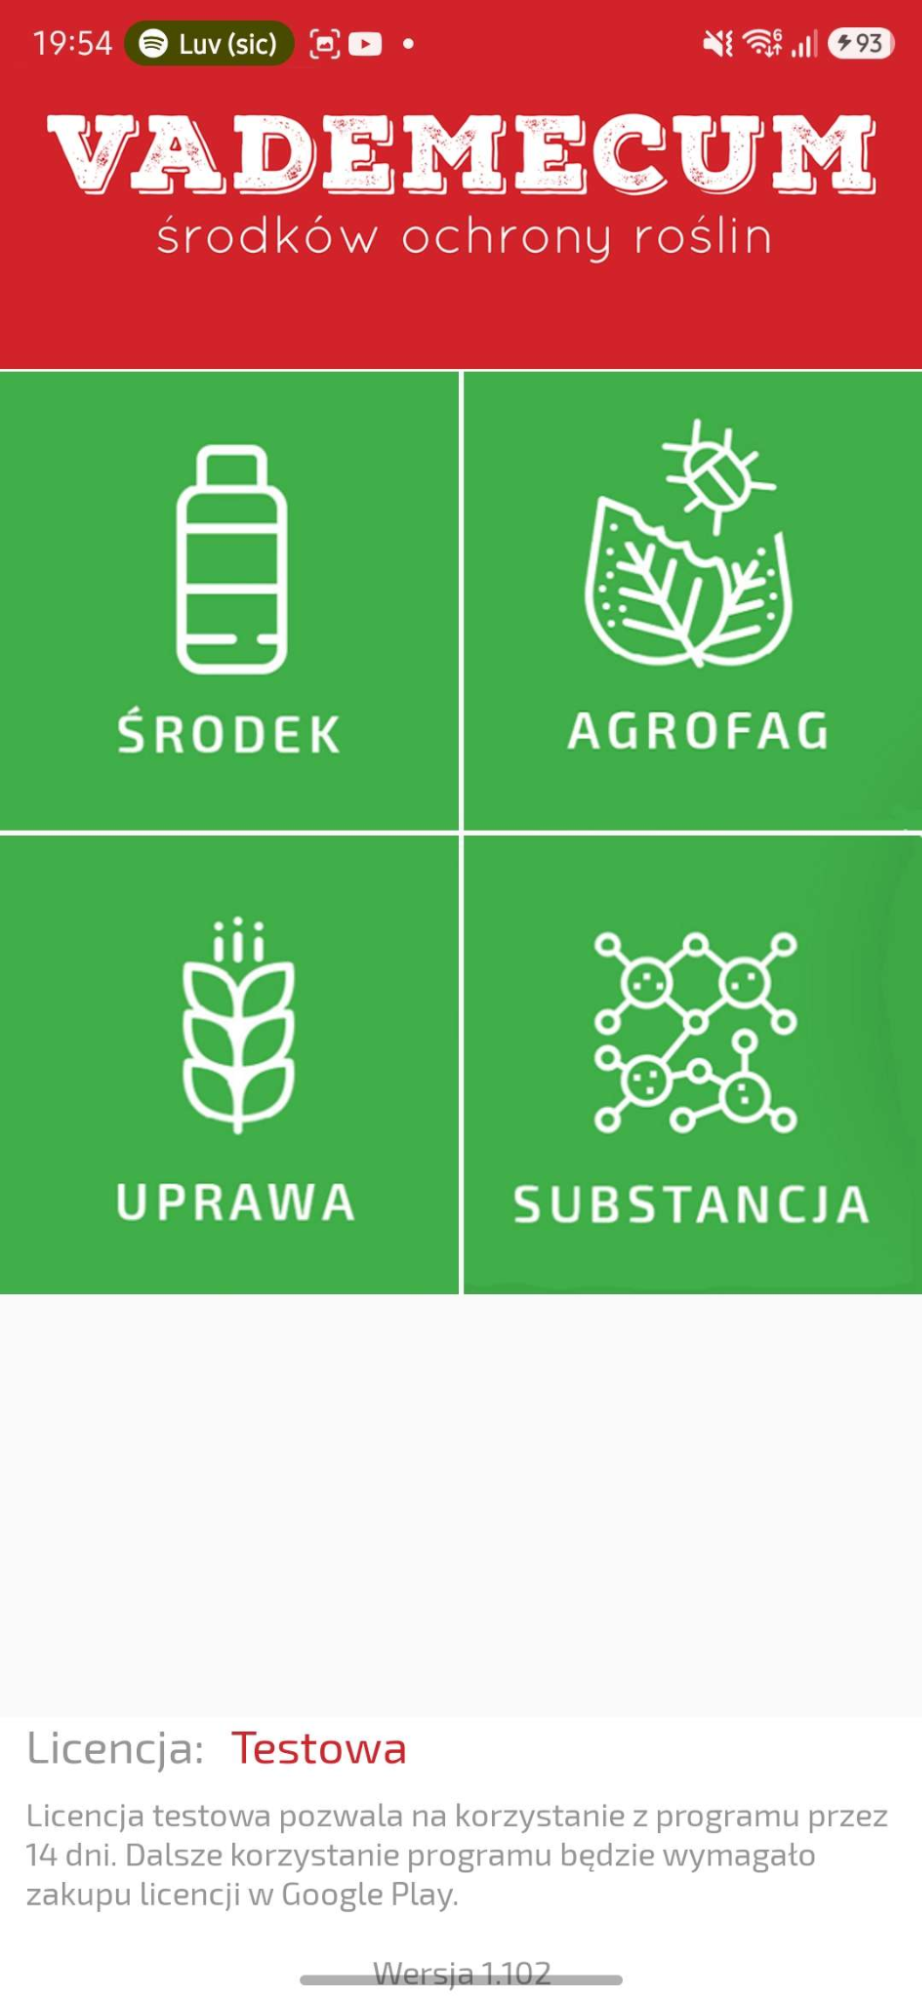
\includegraphics[width=0.3\linewidth]{vademecum1}
    \end{center}

    \item \textbf{Interfejs nieprzystosowany do obsługi w~terenie.}
    Problemy opisano na przykładzie wyszukiwania środka (zrzuty poniżej) --
    pozostałe wyszukiwarki korzystają z~tych samych komponentów.
    Baner reklamowy nachodzi na systemowy pasek stanu, zasłaniając m.in.
    aktualną godzinę. Przyciski powrotu znajdują się bardzo blisko dolnej
    krawędzi ekranu, więc zamiast cofnąć się do menu głównego użytkownik może
    przypadkowo wyjść z~aplikacji. Odstępy między polami wyszukiwania są
    bardzo małe, co zwiększa ryzyko wybrania niewłaściwego pola, a~same pola
    mają niespójny styl (zaokrąglenie tylko po lewej stronie). Przy obsłudze
    telefonu w~kabinie ciągnika takie elementy szczególnie sprzyjają
    pomyłkom.

    \begin{center}
        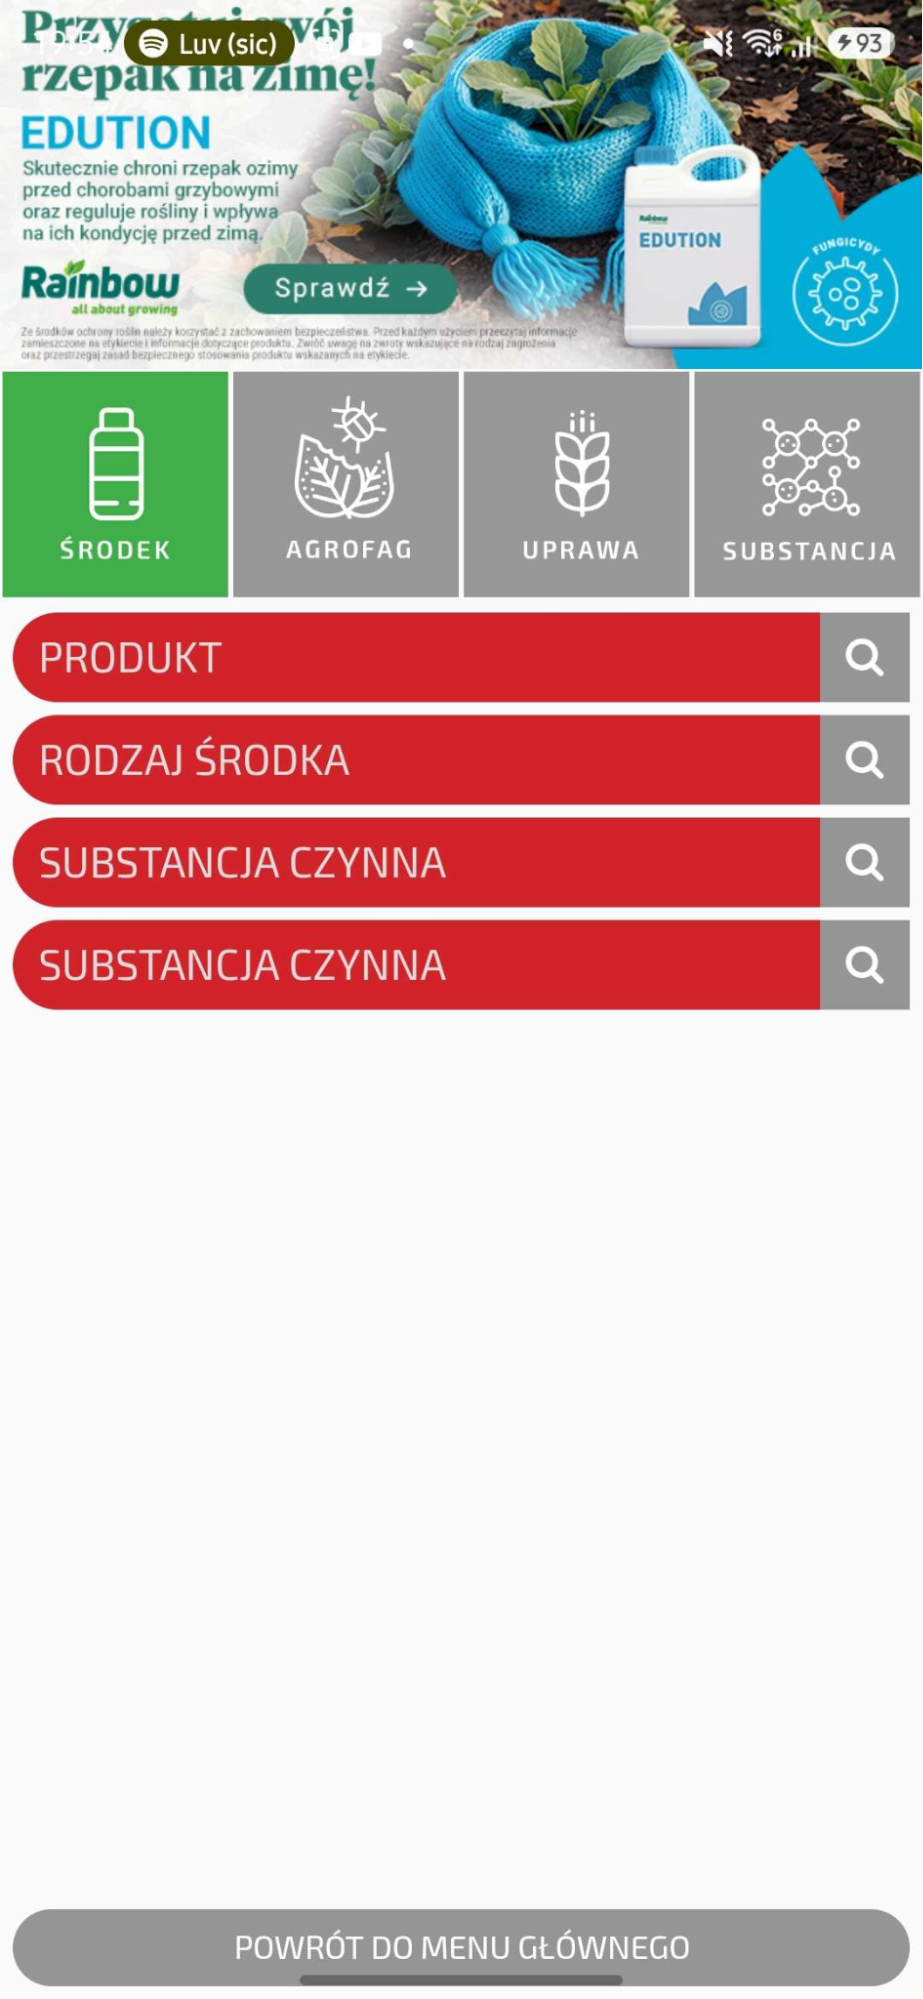
\includegraphics[width=0.3\linewidth]{vademecum2}\hfill
        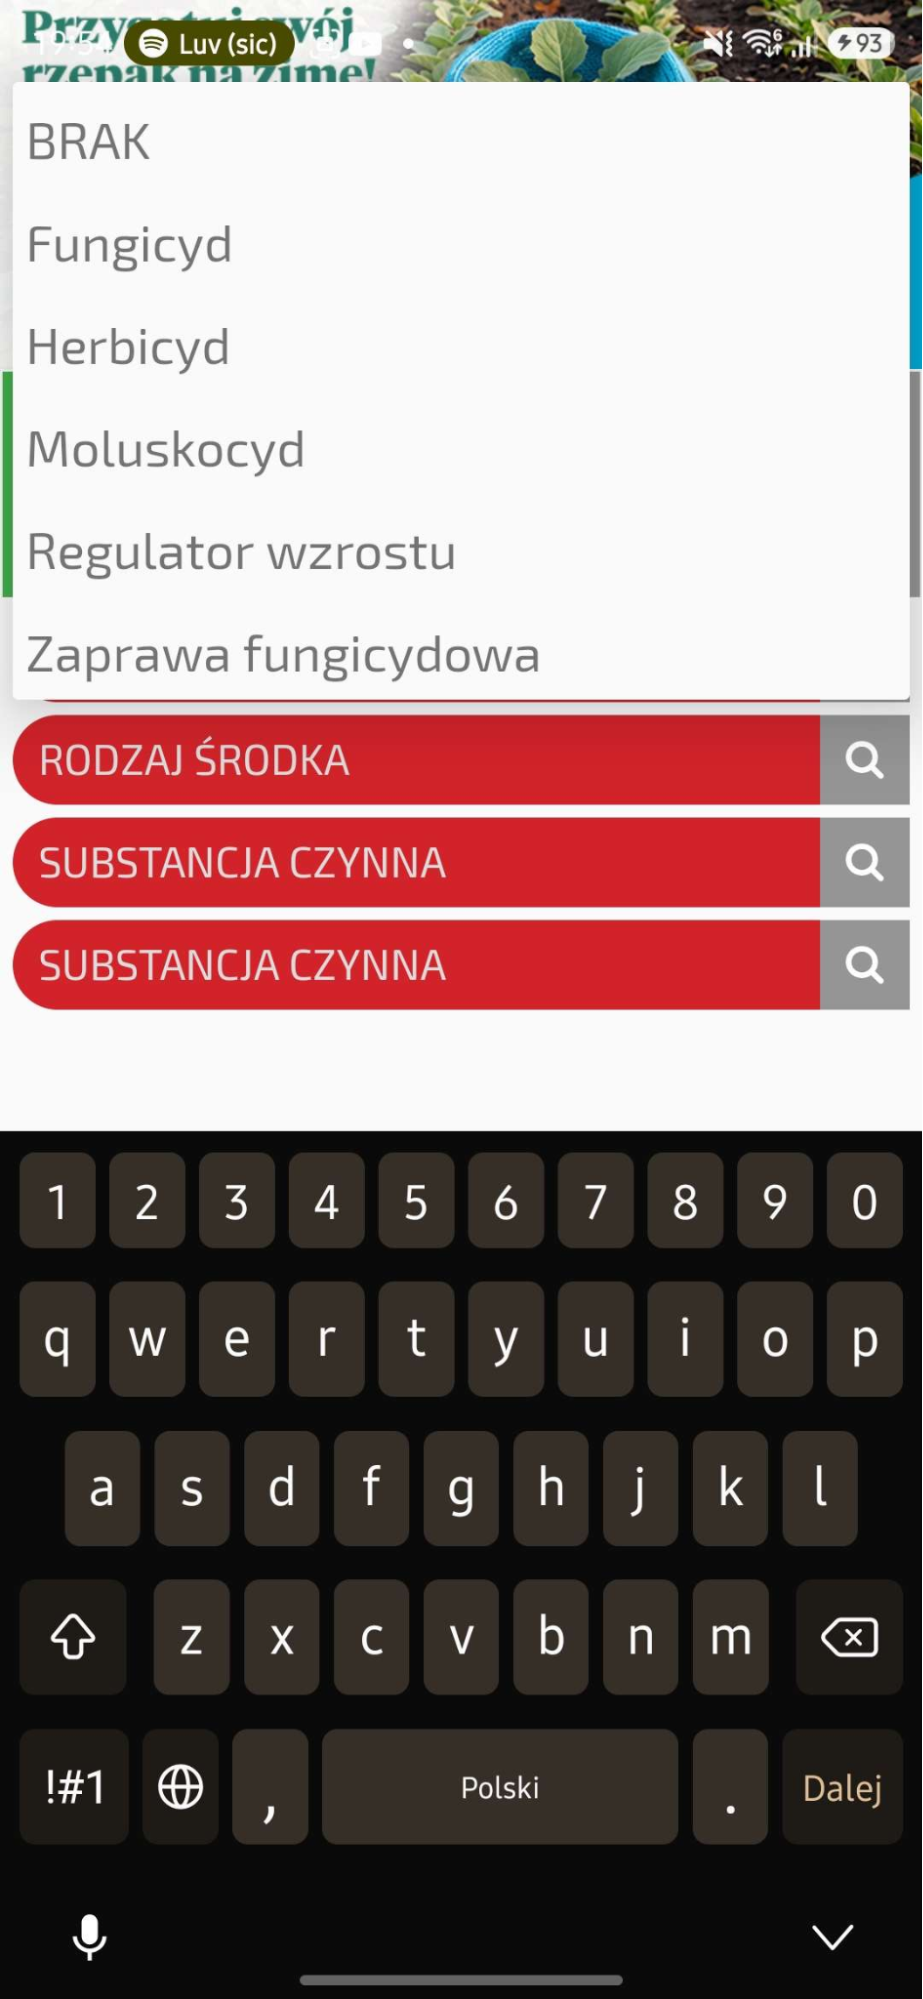
\includegraphics[width=0.3\linewidth]{vademecum3}\hfill
        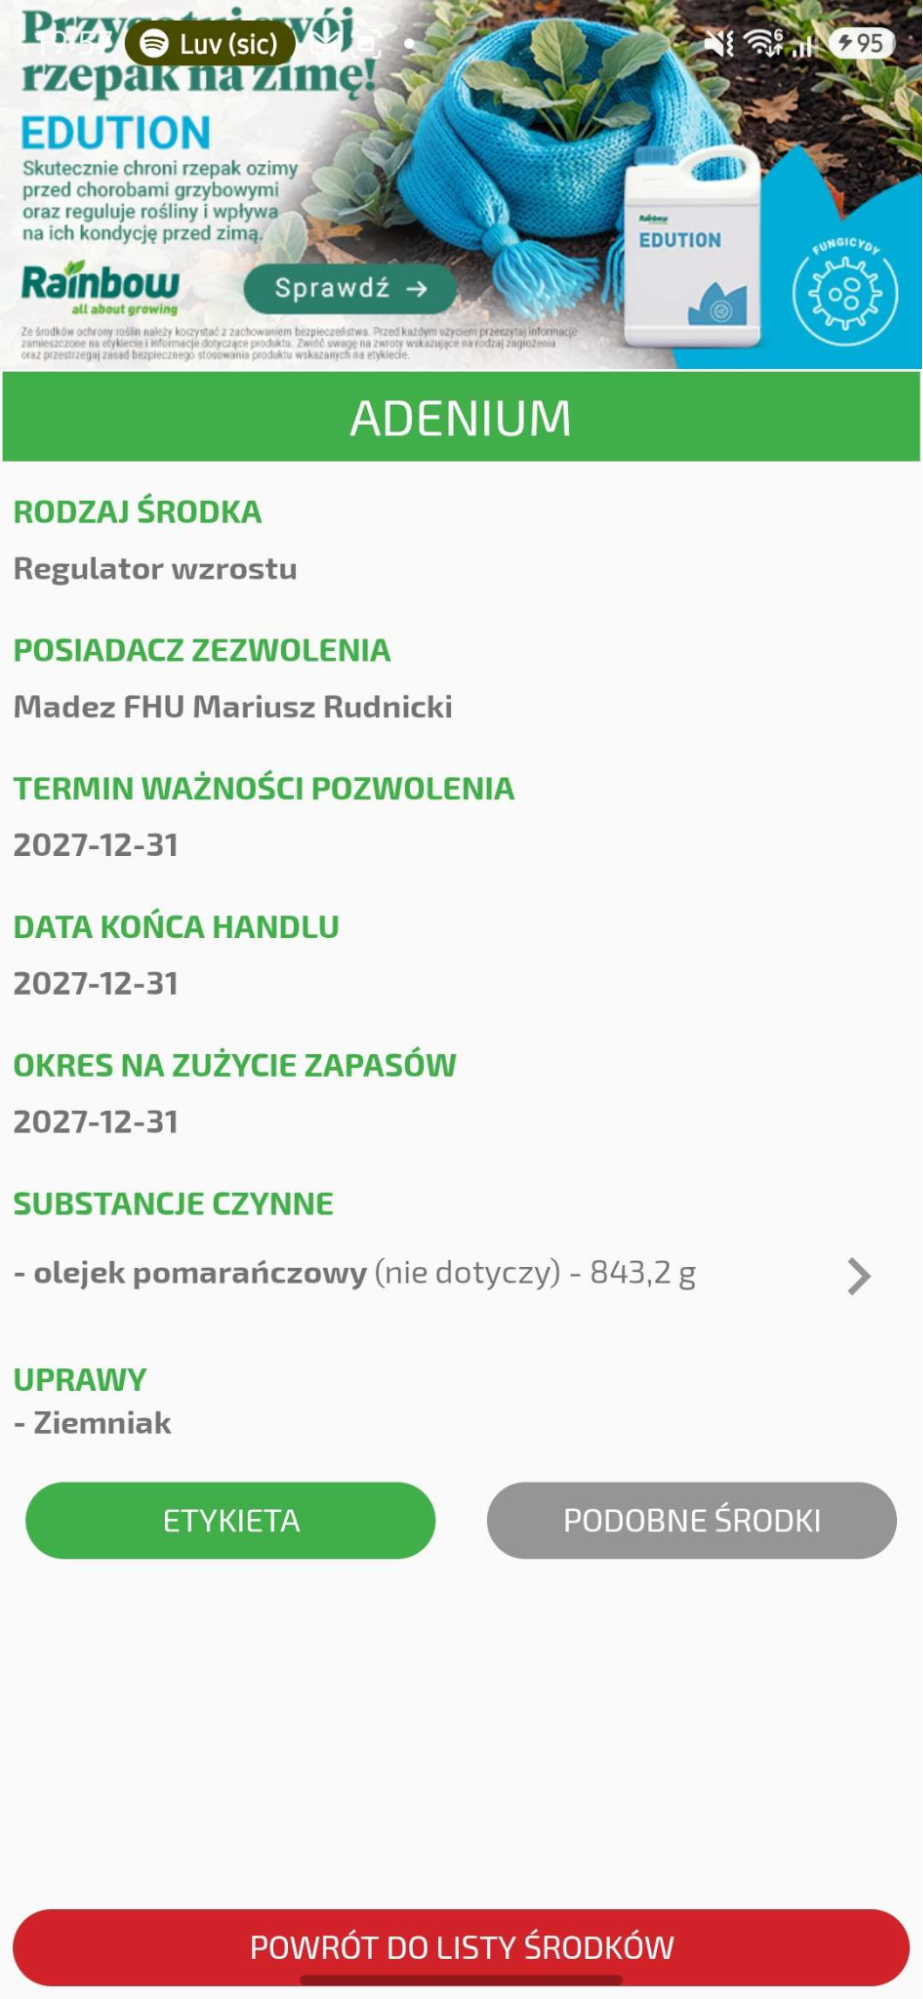
\includegraphics[width=0.3\linewidth]{vademecum4}
    \end{center}

    \item \textbf{Reklamy producentów środków.}
    Aplikacja wyświetla reklamy (w~sklepie Google Play ma oznaczenie
    ,,Zawiera reklamy'') -- na zrzutach widoczny jest baner reklamujący
    środek jednego z~producentów.

    \item \textbf{Etykieta pobierana bez podglądu.}
    Przycisk ,,Etykieta'' od razu pobiera plik na urządzenie, zamiast
    wyświetlić etykietę w~aplikacji z~osobną opcją pobrania. Użytkownik,
    który kilka razy sprawdza tę samą informację, nie wiedząc, że plik został
    już zapisany, może mieć w~telefonie np. cztery kopie tej samej etykiety.

    \item \textbf{Ograniczone możliwości wyszukiwania.}
    Wyszukiwarka nie toleruje literówek, nie pozwala łączyć filtrów (np.
    jednoczesnego wyboru uprawy i~agrofaga) ani ograniczyć wyników do
    środków dla użytkowników nieprofesjonalnych. Karta środka nie zawiera
    też okresu karencji.
\end{itemize}

\subsubsection{Wnioski dla projektu}

\begin{itemize}
    \item \textbf{Zachować:} cztery punkty wejścia do wyszukiwania oraz
    terminy prawne na karcie środka.
    \item \textbf{Nie powtarzać:} ograniczenia do jednej platformy, reklam,
    pobierania etykiety bez podglądu oraz elementów sterujących przy
    krawędziach ekranu.
    \item \textbf{Zrobić lepiej:} bezpłatny dostęp w~przeglądarce, podgląd
    etykiety w~aplikacji, okres karencji na karcie środka, duże elementy
    dotykowe z~odstępami oraz wyszukiwanie odporne na literówki z~możliwością
    łączenia filtrów.
\end{itemize}

\subsection{Wyszukiwarka środków ochrony roślin Ministerstwa Rolnictwa}

\subsubsection{Opis rozwiązania}

Ministerstwo Rolnictwa i~Rozwoju Wsi udostępnia na portalu gov.pl bezpłatną
wyszukiwarkę środków ochrony roślin. Według opisu ministerstwa pozwala ona
wyszukiwać środki ,,przede wszystkim po uprawach i~agrofagach'', a~także po
substancji czynnej, rodzaju środka oraz zastosowaniach
małoobszarowych.
Wyniki prezentowane są w~formie tabeli z~12 kolumnami, w~której każdy wiersz
opisuje jedno zastosowanie środka (środek, uprawa i~agrofag). Tabela zawiera
m.in. numer zezwolenia, rodzaj środka, substancję czynną z~zawartością, metodę
stosowania oraz rodzaj użytkownika (profesjonalny lub amatorski). Pozostałe
informacje -- terminy ważności zezwolenia i~dopuszczenia do sprzedaży
i~stosowania, dawka oraz termin stosowania -- są dostępne dopiero po wybraniu
opcji ,,zobacz szczegóły'' przy danym wierszu. Ministerstwo
udostępnia również plik źródłowy wyszukiwarki w~formacie XLSX, a~etykiety
środków -- na osobnej podstronie portalu. Formularz wyszukiwarki z~rozwiniętymi
filtrami przedstawiono poniżej.

\begin{center}
    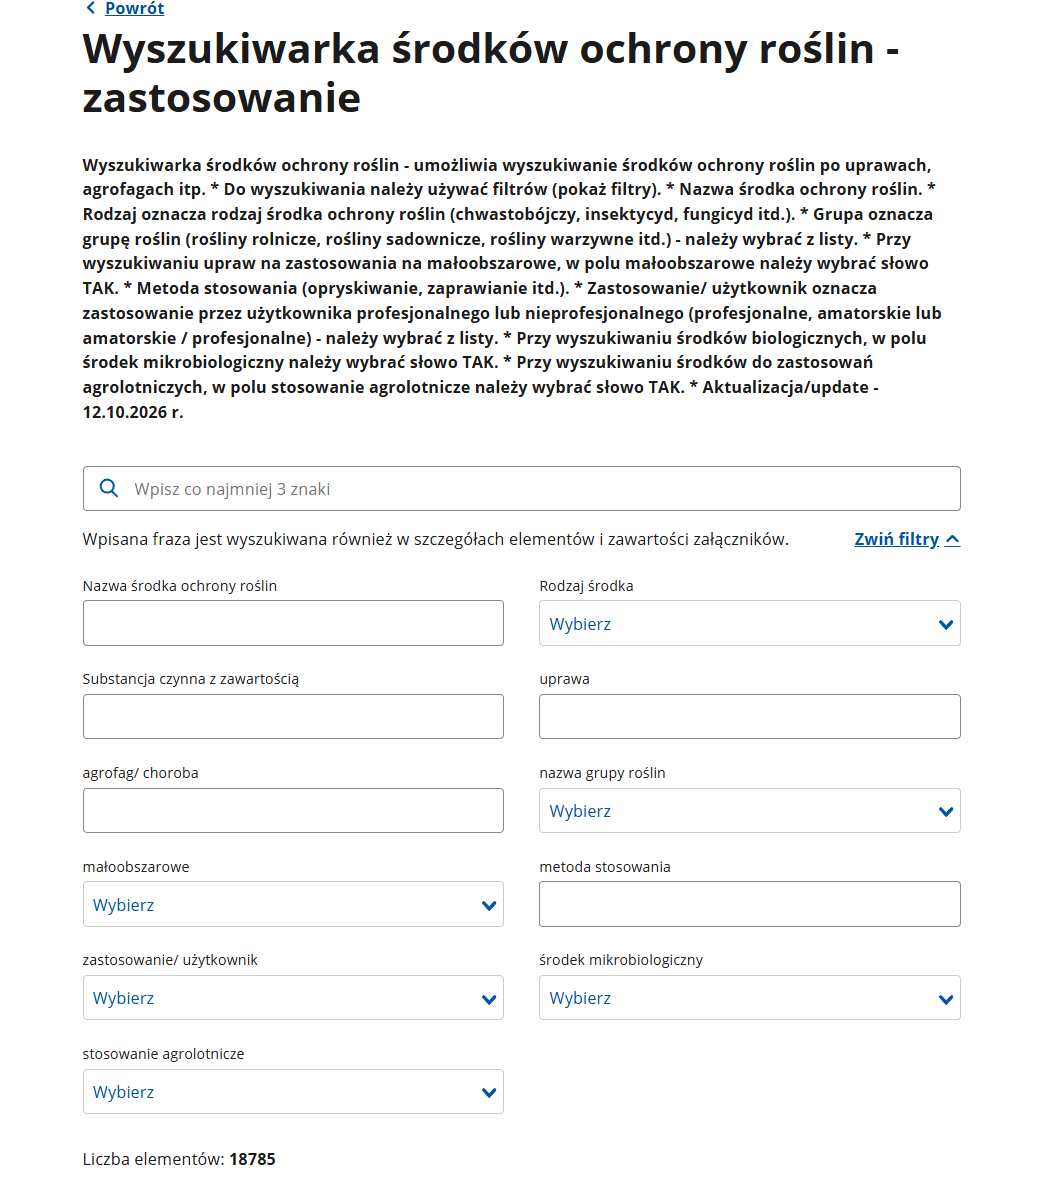
\includegraphics[width=0.72\textwidth]{GOV1}
\end{center}

\subsubsection{Mocne strony}

\begin{itemize}
    \item \textbf{Oficjalne i~bezpłatne źródło danych.}
    Dane pochodzą bezpośrednio od organu wydającego zezwolenia, a~korzystanie
    z~wyszukiwarki nie wymaga instalacji, logowania ani opłat.

    \item \textbf{Łączenie kryteriów wyszukiwania.}
    Większość kolumn ma własne pole filtra, dzięki czemu można jednocześnie
    zawęzić wyniki np. do konkretnej uprawy, agrofaga i~rodzaju środka.

    \item \textbf{Informacja o~rodzaju użytkownika.}
    Kolumna ,,zastosowanie/ użytkownik'' pozwala ograniczyć wyniki do
    zastosowań dopuszczonych dla użytkowników nieprofesjonalnych. W~danych
    pobranych 12~października 2026~r. na ok.~18,8~tys. zastosowań 346
    oznaczono jako wyłącznie amatorskie, a~ok.~1,5~tys. jako amatorskie
    i~profesjonalne.

    \item \textbf{Widoczna data aktualizacji.}
    W~opisie nad formularzem podana jest data ostatniej aktualizacji danych
    (12.10.2026~r.), dzięki czemu użytkownik wie, czy korzysta z~aktualnych
    informacji.
\end{itemize}

\subsubsection{Słabe strony}

\begin{itemize}
    \item \textbf{Pobieranie całej bazy przy każdym otwarciu.}
    Strona wyszukiwarki zawiera wszystkie zastosowania środków -- w~dniu
    analizy miała rozmiar ok.~10~MB. Przy słabym zasięgu w~polu wydłuża to
    wczytywanie strony i~zużywa pakiet danych użytkownika.

    \item \textbf{Zwielokrotnione wyniki.}
    Ministerstwo samo zaznacza, że ponieważ wyszukiwarka jest ,,zaprojektowana
    głównie pod uprawy'', w~wynikach ,,mogą pojawiać się zwielokrotnione nazwy
    środków ochrony roślin''. Użytkownik szukający informacji o~jednym środku
    musi przeglądać wiele wierszy zamiast jednej karty środka. Na zrzucie
    poniżej środek 3C-750 zajmuje sześć kolejnych wierszy -- po jednym dla
    każdej uprawy. Domyślnie wyświetlanych jest 10 wierszy na stronę, co przy
    18\,785 zastosowaniach daje 1879 stron wyników.

    \begin{center}
        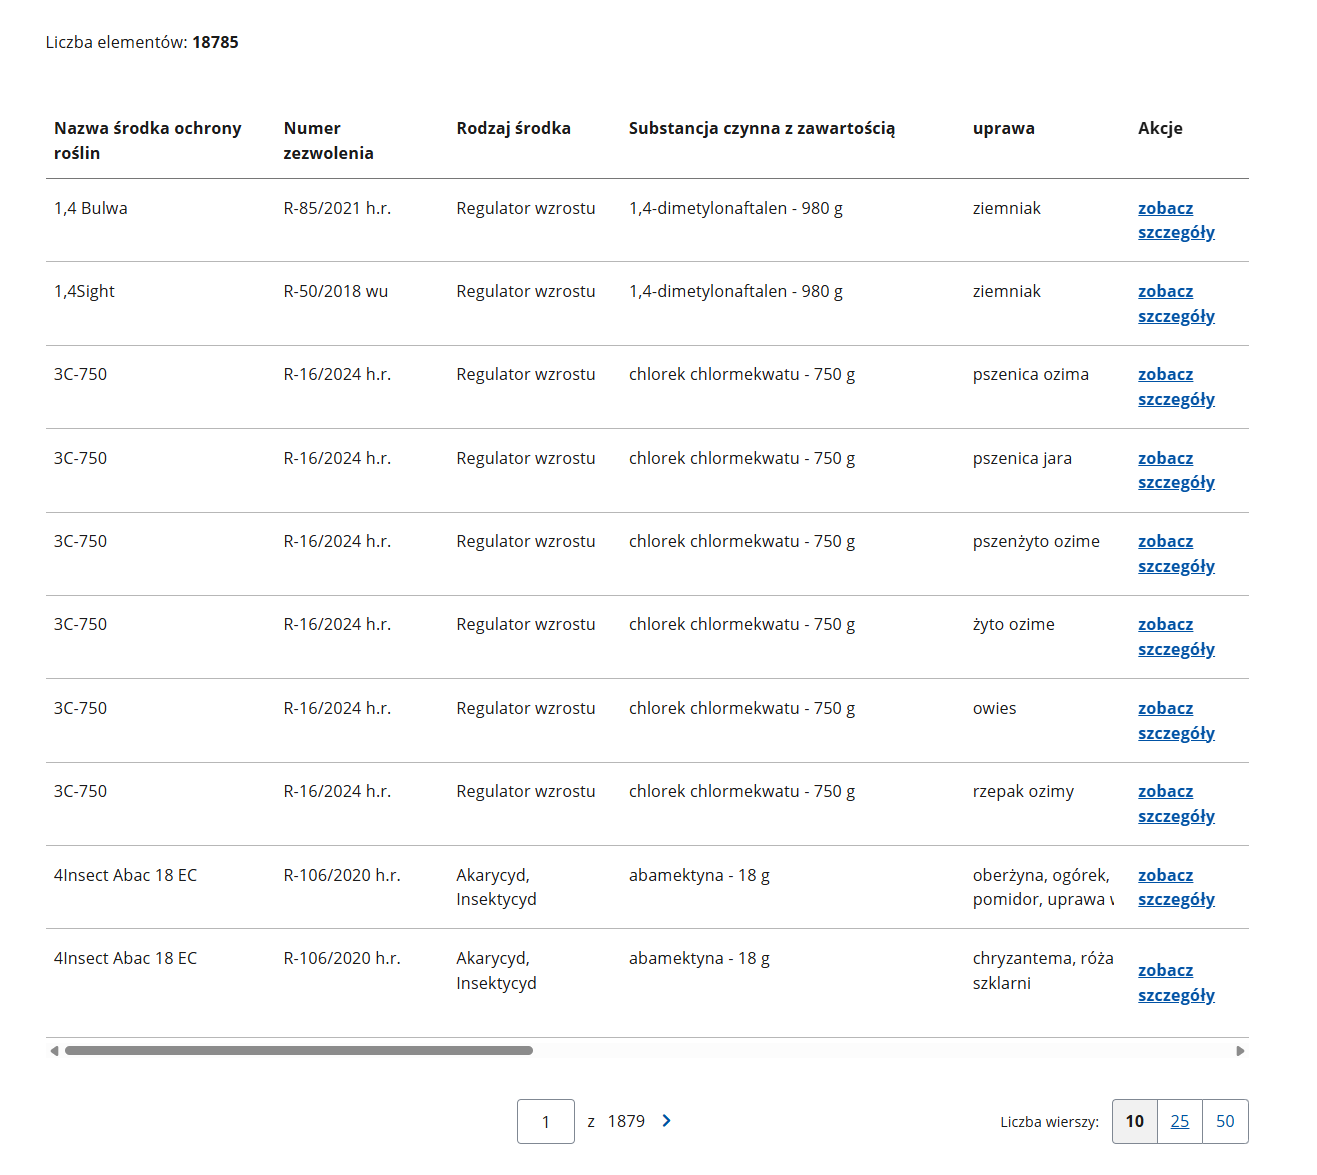
\includegraphics[width=0.85\textwidth]{GOV2}
    \end{center}

    \item \textbf{Etykieta poza wynikami.}
    Wyniki nie zawierają odnośników do etykiet -- aby zapoznać się z~etykietą,
    użytkownik musi przejść na osobną stronę z~etykietami i~odnaleźć tam
    właściwy dokument. Okres karencji jest podawany w~karcie produktu.
    Widok szczegółów pojedynczego zastosowania przedstawiono poniżej.

    \begin{center}
        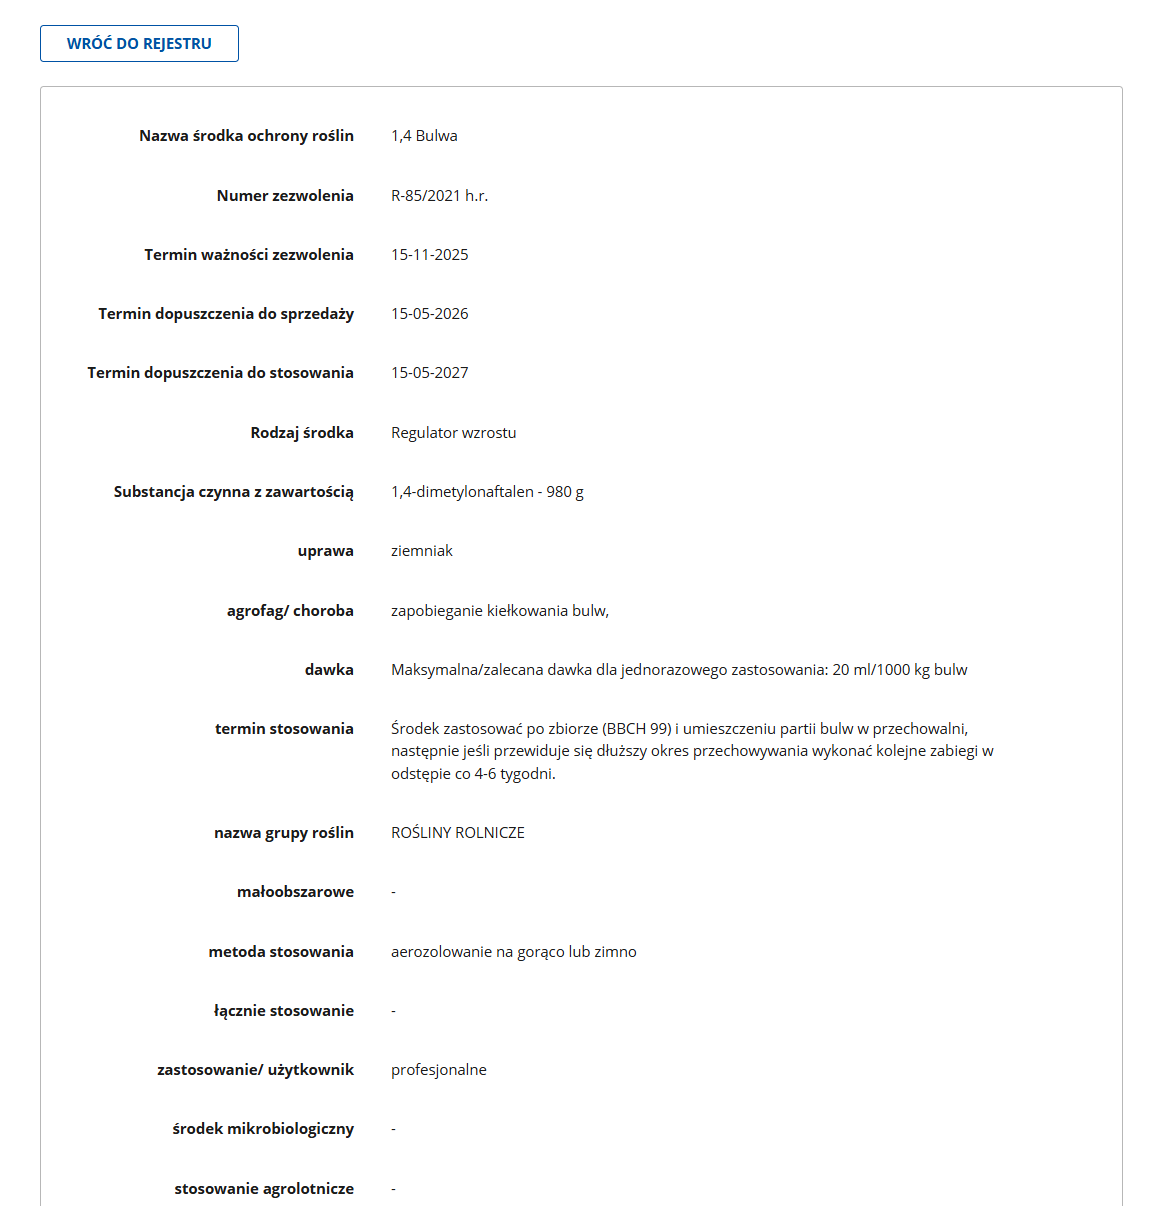
\includegraphics[width=0.85\linewidth]{GOV3}
    \end{center}

    \item \textbf{Tabela szersza niż ekran.}
    Tabela wyników nie mieści się w~całości nawet na monitorze komputera
    i~wymaga przewijania w~poziomie. Na zrzutach poniżej przedstawiono tę samą
    stronę wyników po przewinięciu tabeli do środka i~do prawej krawędzi.
    Kolumna ,,zastosowanie/ użytkownik'', kluczowa dla ogrodnika amatora,
    jest widoczna dopiero po przewinięciu tabeli do samego końca.

    \begin{center}
        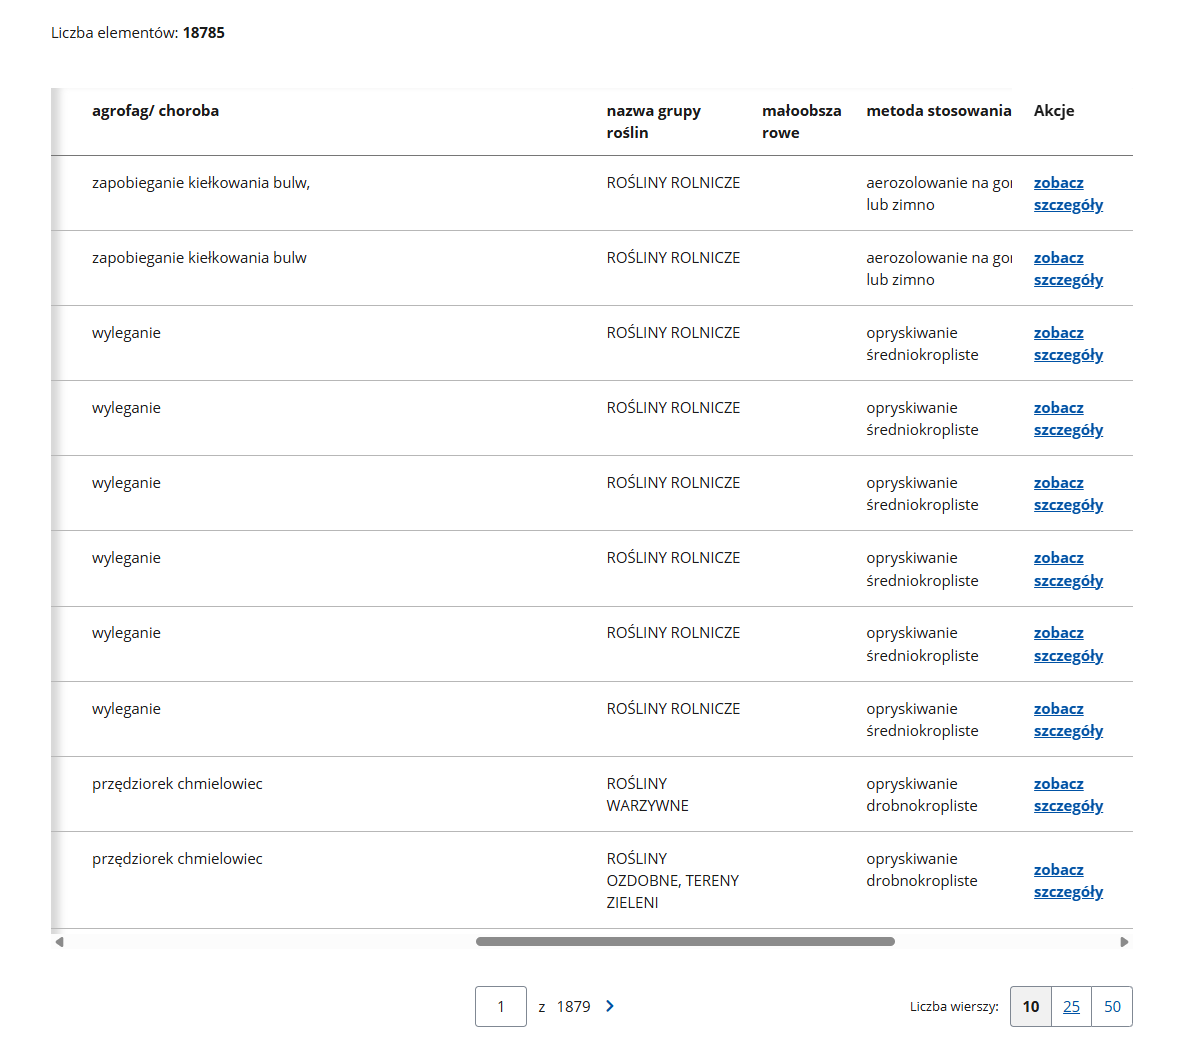
\includegraphics[width=0.9\linewidth]{GOV5}

        \vspace{0.5em}
        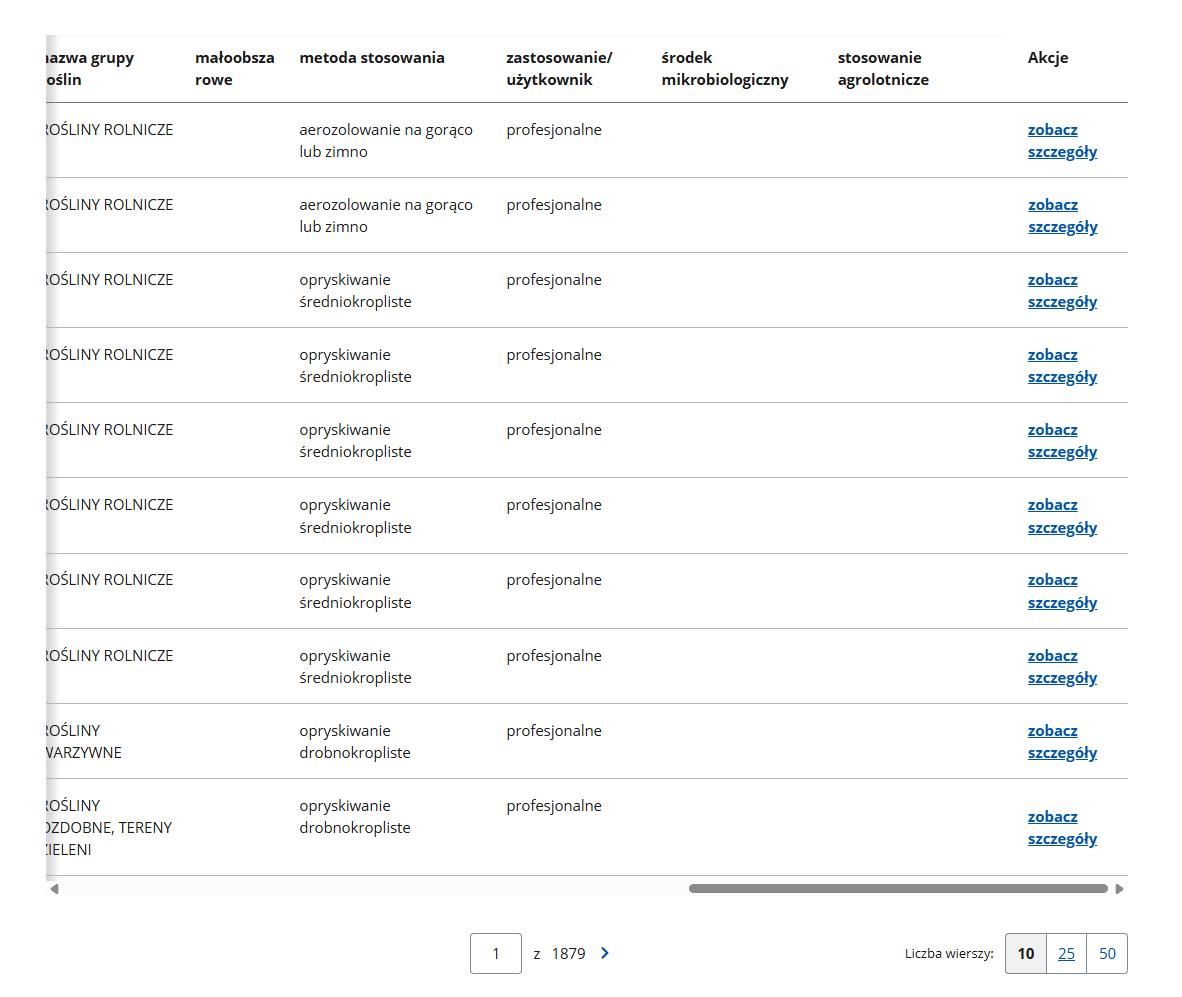
\includegraphics[width=0.9\linewidth]{GOV6}
    \end{center}

    \newpage
    Na ekranie telefonu problem jest jeszcze wyraźniejszy: widoczne są
    jedynie dwie pierwsze kolumny tabeli (nazwa środka i~numer zezwolenia),
    a~pozostałe, w~tym rodzaj środka i~uprawa, wymagają przewijania
    w~poziomie. Ponadto nad wynikami znajduje się formularz kilkunastu
    filtrów, który trzeba przewinąć, aby dotrzeć do tabeli.

    \begin{center}
        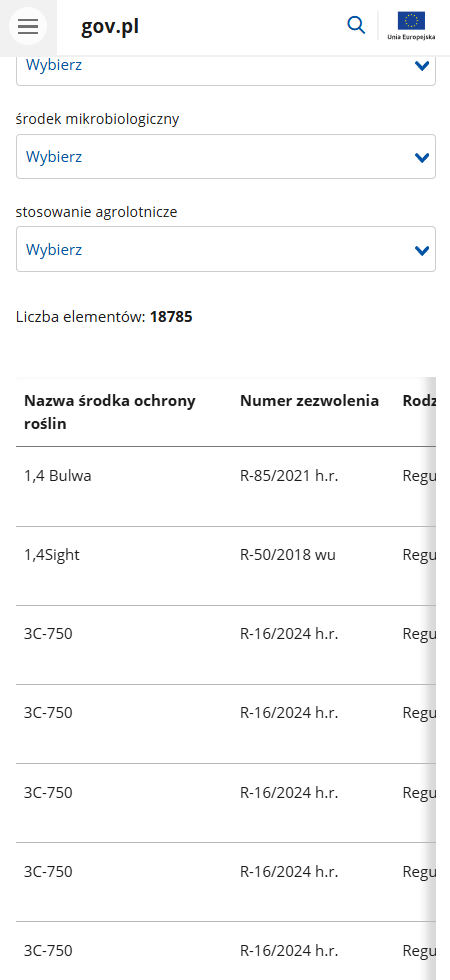
\includegraphics[height=12cm]{GOV4}
    \end{center}

    \item \textbf{Brak tolerancji literówek.}
    Wyszukiwarka dopasowuje wyłącznie dokładnie wpisany fragment tekstu.
    Podczas testów wpisanie nazwy środka z~literówką nie pozwoliło go
    odnaleźć. Jest to szczególnie uciążliwe przy nazwach handlowych, które
    często zawierają cyfry, skróty i~nietypową pisownię (np. ,,1,4Sight'',
    ,,3C-750'').
\end{itemize}

\subsubsection{Wnioski dla projektu}

\begin{itemize}
    \item \textbf{Zachować:} osobne filtry dla uprawy, agrofaga i~rodzaju
    środka oraz informację o~rodzaju użytkownika. Pliki CSV/XLSX publikowane
    przez ministerstwo na portalu dane.gov.pl mogą posłużyć jako źródło
    danych dla mechanizmu automatycznej aktualizacji.
    \item \textbf{Nie powtarzać:} przesyłania całej bazy do przeglądarki
    oraz wielokrotnego wyświetlania tego samego środka.
    \item \textbf{Zrobić lepiej:} wyniki pogrupowane według środka, karta
    środka z~odnośnikiem do etykiety i~wyróżnionym okresem karencji.
\end{itemize}

\newpage
\subsection{AgroBase}

\subsubsection{Opis rozwiązania}

AgroBase to międzynarodowa aplikacja litewskiej firmy Farmis, łącząca bazę
wiedzy o~agrofagach (chwastach, chorobach i~szkodnikach) z~bazą środków
ochrony roślin zarejestrowanych w~wybranym kraju. Jest dostępna na Androida
(ponad 500~tys. pobrań w~sklepie Google Play) i~iOS oraz w~wersji
przeglądarkowej z~osobną sekcją dla Polski. Interfejs obsługuje 45 języków,
w~tym polski. Wyszukiwarka w~podstawowej wersji jest bezpłatna i~zawiera
reklamy. Dodatkowe funkcje, takie jak lista ostatnio wybieranych środków,
wymagają subskrypcji w~cenie 16,99~zł miesięcznie lub 5,25~zł miesięcznie
przy płatności za rok z~góry. Jest to subskrypcja samej wyszukiwarki, a~nie
całego systemu AgroBase.

Użytkownik może wyszukać środek po nazwie, substancji czynnej, kategorii
lub uprawie albo zacząć od rozpoznania agrofaga na podstawie opisów
i~zdjęć, a~następnie przejść do środków, które go zwalczają. Karta środka
zawiera m.in. producenta, numer rejestracyjny, datę ważności rejestracji,
substancję czynną, odnośnik do etykiety oraz tabelę upraw z~dawką,
terminem stosowania (BBCH) i~okresem karencji. Dostępna jest także funkcja
porównania środków oraz zgłaszania błędów w~danych.

\subsubsection{Mocne strony}

\begin{itemize}
    \item \textbf{Wszystkie kluczowe informacje na jednej karcie.}
    Dawka, termin stosowania i~okres karencji są przedstawione w~jednej
    tabeli dla każdej uprawy, a~karta środka zawiera odnośnik do etykiety
    (choć nie zawsze działający -- zob. słabe strony). W~Vademecum etykietę
    trzeba pobrać jako plik, a~okresu karencji na karcie środka nie ma.
    W~wyszukiwarce ministerstwa okres karencji jest podawany w~karcie
    produktu, ale etykieta znajduje się na osobnej stronie.

    \item \textbf{Powiązanie agrofaga ze środkiem.}
    Rolnik, który nie zna nazwy szkodnika lub choroby, może najpierw
    rozpoznać go na podstawie zdjęć i~opisu, a~dopiero potem wyszukać
    środki, które go zwalczają.

    \item \textbf{Trzy platformy.}
    Aplikacja działa na Androidzie, iOS oraz w~przeglądarce.
\end{itemize}

\subsubsection{Słabe strony}

\begin{itemize}
    \item \textbf{Tłumaczenie maszynowe.}
    Polskie teksty zawierają błędy wskazujące na automatyczne tłumaczenie,
    np. na karcie środka ,,Aktywne materiały'' zamiast ,,substancje
    czynne'', ,,Stawka'' zamiast ,,dawka'' czy ,,Karencji interwał'',
    a~w~opisie aplikacji w~sklepie Google Play ,,Dokonywanie harcerstwa
    w~terenie'' (z~ang. \emph{scouting} -- lustracja pól). Terminologia
    niezgodna z~etykietami utrudnia zrozumienie danych i~obniża zaufanie
    do nich.

    \item \textbf{Wątpliwa jakość części danych.}
    Na karcie środka Amistar 250 SC dla słodkiej papryki podano dawkę
    ,,0~l'', co wskazuje na błąd w~danych. Aplikacja nie jest oficjalnym
    źródłem, a~producent sam prosi użytkowników o~zgłaszanie błędnych
    informacji.

    \item \textbf{Nieaktualna baza środków.}
    Polska sekcja wersji przeglądarkowej zawiera 1797 środków. Porównanie
    ich nazw z~danymi wyszukiwarki ministerstwa, przeprowadzone
    13~października 2026~r., wykazało, że w~aktualnym rejestrze występuje jedynie od 935 do ok.~1130
    z~nich (52--63\,\%, zależnie od sposobu dopasowania nazw). Pozostałych
    środków nie ma w~aktualnym rejestrze -- na stronie głównej listy
    wyświetlane są np. Arcade 880 EC, którego rejestracja według samej
    aplikacji wygasła 4~marca 2026~r., oraz Maxim Star 025 FS, również
    z~wygasłą rejestracją. Aplikacja nie pozwala odfiltrować takich środków.
    Jednocześnie aktywne środki w~AgroBase to zaledwie ok.~jedna trzecia
    z~ok.~3~tys. środków występujących w~danych ministerstwa, więc
    użytkownik może nie znaleźć w~aplikacji środka, który jest dopuszczony
    do stosowania.

    \item \textbf{Nieneutralna kolejność środków.}
    Lista środków nie jest uporządkowana alfabetycznie -- na jej początku
    wyświetlane są produkty firm Bayer i~Syngenta. Na zrzucie poniżej
    widać początek listy: pierwszym środkiem jest Arcade 880 EC z~wygasłą
    rejestracją, a~kolejne pozycje to wyłącznie produkty tych dwóch firm.

    \begin{center}
        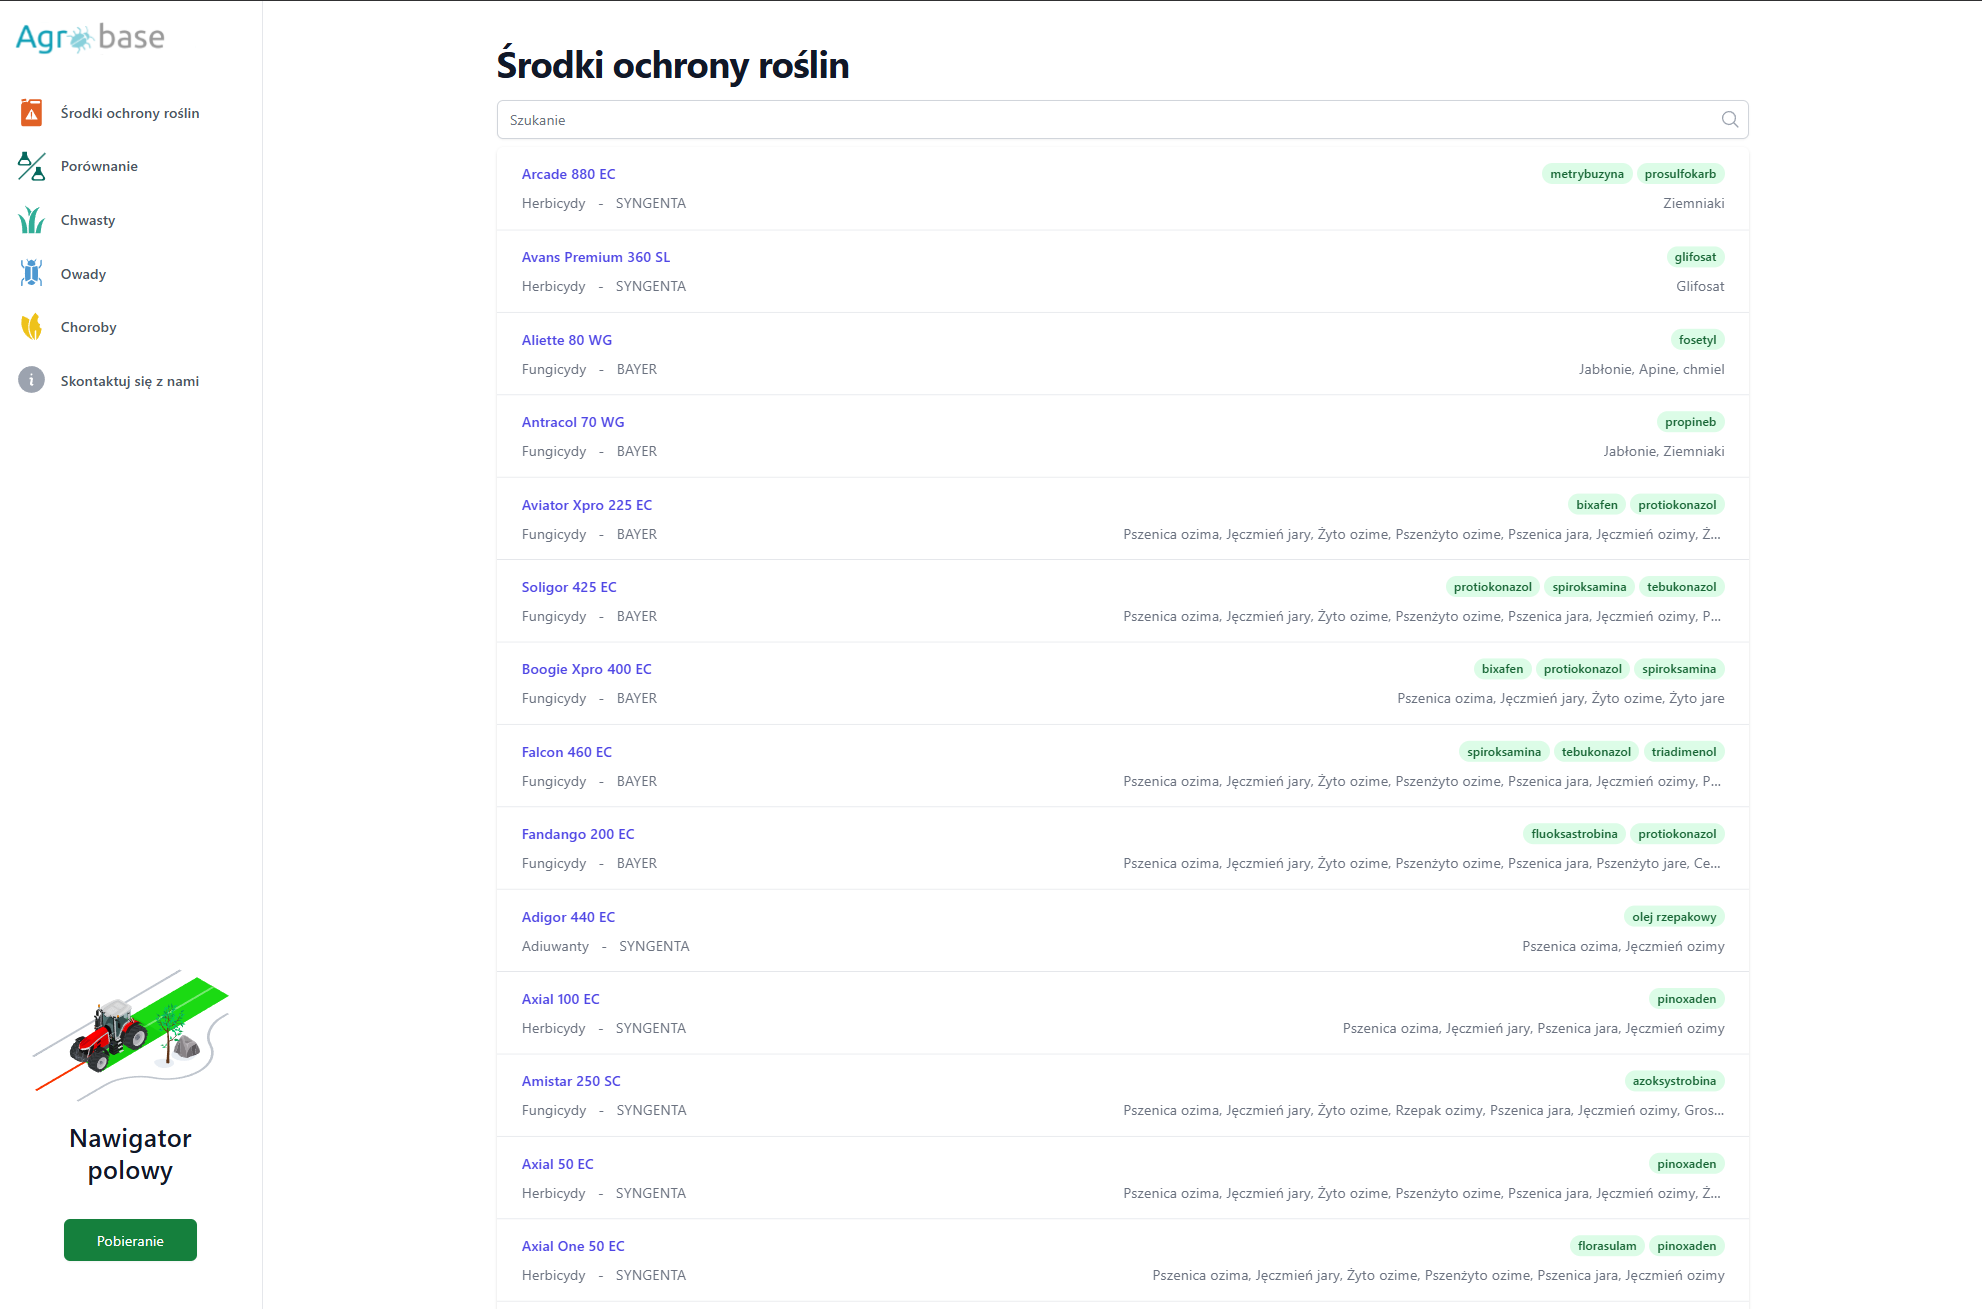
\includegraphics[width=\linewidth]{AgroBase1}
    \end{center}

    \item \textbf{Niedziałające odnośniki do etykiet.}
    Odnośniki do etykiet i~kart charakterystyki prowadzą do różnych
    serwisów -- części do portalu gov.pl, części do stron producentów.
    Odnośniki do strony firmy Bayer zwracają błąd 404 (strona nie
    istnieje), np. etykieta środka Antracol 70 WG oraz karta
    charakterystyki środka Aliette 80 WG. Karta tego ostatniego środka
    (poniżej) pokazuje jednocześnie inne opisane problemy: datę wygaśnięcia
    rejestracji (14~marca 2026~r.) aplikacja wyróżnia kolorem czerwonym,
    ale nadal prezentuje środek, a~substancja czynna opisana jest jako
    ,,Aktywne materiały''.

    \begin{center}
        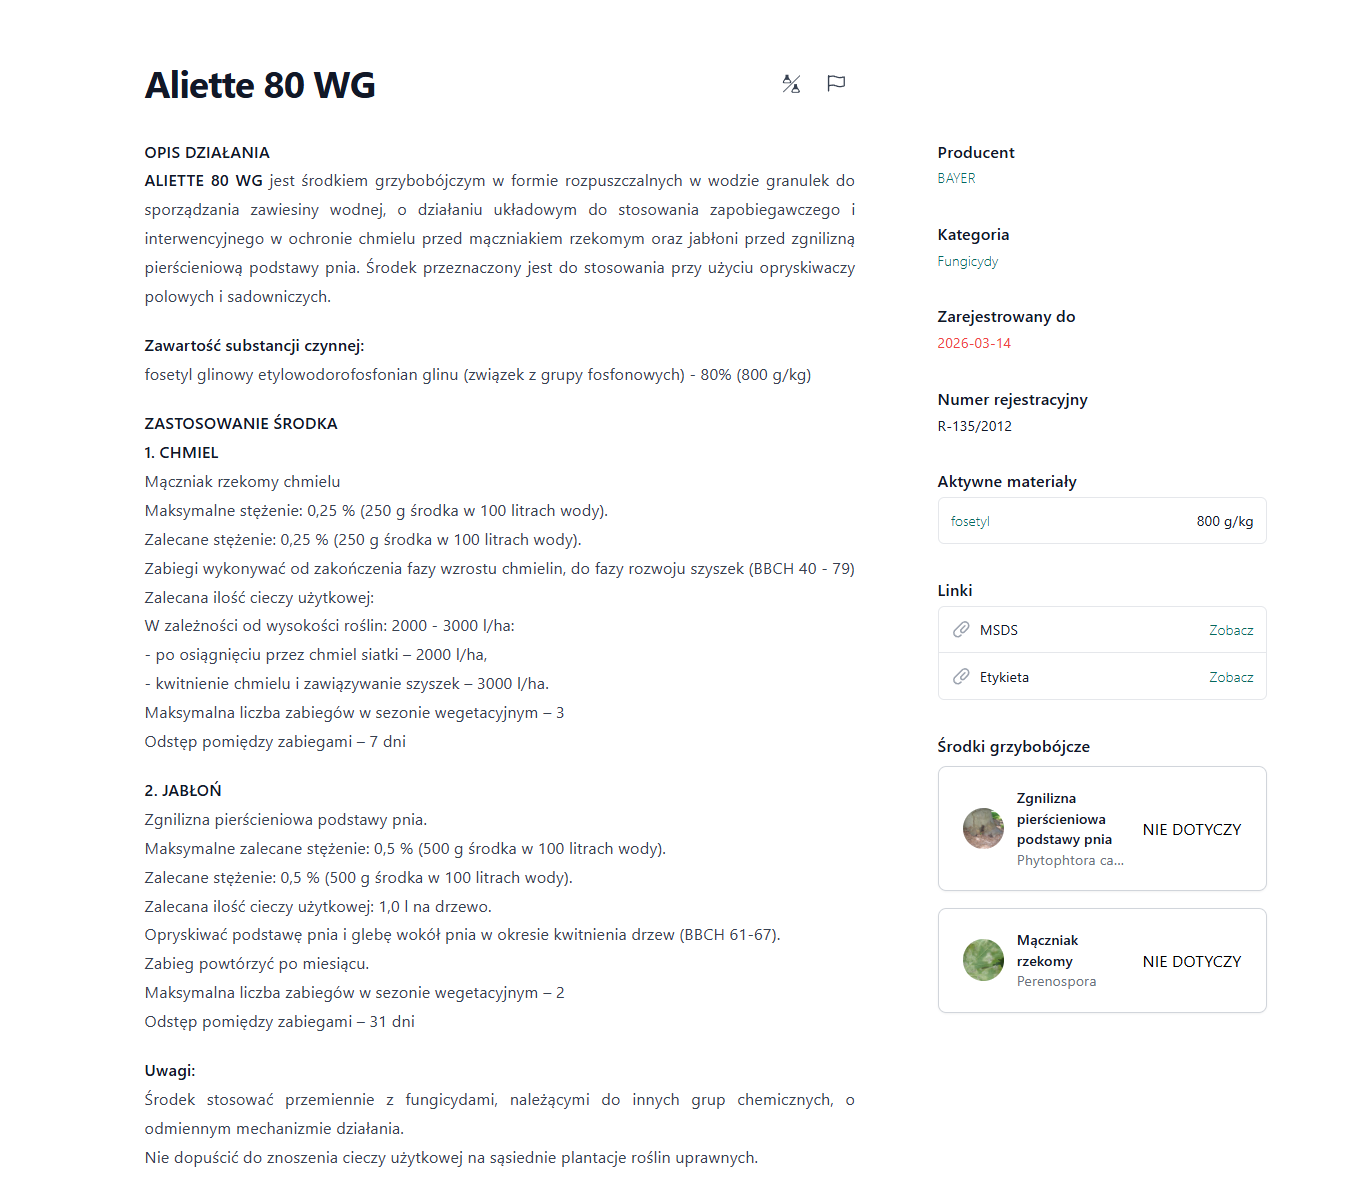
\includegraphics[width=\linewidth]{AgroBase2}
    \end{center}

    \item \textbf{Niepełne informacje prawne.}
    Karta środka podaje jedynie datę ważności rejestracji -- brakuje
    terminów dopuszczenia do sprzedaży i~stosowania, które są dostępne
    w~Vademecum i~w~wyszukiwarce ministerstwa.

    \item \textbf{Ograniczone możliwości wyszukiwania.}
    Wyszukiwarka nie toleruje literówek, nie pozwala łączyć filtrów
    (np. jednoczesnego wyboru uprawy i~agrofaga) ani ograniczyć wyników do
    środków dopuszczonych dla użytkowników nieprofesjonalnych.

    \item \textbf{Reklamy i~płatne subskrypcje.}
    Bezpłatna wersja wyświetla reklamy, a~nawet tak podstawowe udogodnienia
    jak lista ostatnio wybieranych środków wymagają subskrypcji (16,99~zł
    miesięcznie lub 5,25~zł miesięcznie przy płatności rocznej).
\end{itemize}

\subsubsection{Wnioski dla projektu}

\begin{itemize}
    \item \textbf{Zachować:} kartę środka z~tabelą upraw zawierającą dawkę
    i~okres karencji oraz możliwość zgłoszenia błędu w~danych.
    \item \textbf{Nie powtarzać:} tłumaczenia maszynowego -- interfejs
    powinien używać terminologii zgodnej z~etykietami (substancja czynna,
    dawka, okres karencji).
    \item \textbf{Zrobić lepiej:} dane pobierane bezpośrednio z~oficjalnego
    źródła (ministerstwa) i~regularnie aktualizowane, tak aby nie
    wyświetlać środków z~wygasłą rejestracją; pełne terminy prawne, data
    aktualizacji oraz etykiety pochodzące z~portalu gov.pl zamiast
    z~zewnętrznych serwisów producentów.
\end{itemize}

\subsection{Porównanie funkcji}

\begin{center}
\footnotesize
\begin{tabular}{|p{3.5cm}|p{2.8cm}|p{2.8cm}|p{2.5cm}|p{1.9cm}|}
\hline
\textbf{Funkcja} & \textbf{Vademecum} & \textbf{MRiRW} & \textbf{AgroBase} & \textbf{Projekt} \\
\hline
Platformy & Android & przeglądarka & Android, iOS, przeglądarka & przeglądarka \\
\hline
Koszt & 119 zł/rok (odnowienie 139 zł) lub 829 zł & bezpłatne & bezpłatne z~reklamami; subskrypcja 16,99~zł/mies. lub 5,25~zł/mies. rocznie & bezpłatne \\
\hline
Wyszukiwanie po nazwie, uprawie, agrofagu, substancji & tak & tak & tak & tak \\
\hline
Łączenie filtrów (uprawa + agrofag) & nie & tak & nie & tak \\
\hline
Tolerancja literówek & nie & nie & nie & tak \\
\hline
Filtr środków dla amatorów & nie & tak & nie & tak \\
\hline
Podgląd etykiety w~aplikacji & nie (pobranie pliku) & nie (osobna strona) & nie (odnośnik zewnętrzny, część nie działa) & tak \\
\hline
Okres karencji na karcie środka & nie & tak & tak & tak \\
\hline
Terminy prawne & tak & tak & tylko ważność rejestracji & tak \\
\hline
Reklamy & tak & nie & tak & nie \\
\hline
\end{tabular}
\end{center}

Różnice w~funkcjach wynikają przede wszystkim z~celu, w~jakim powstało każde
z~rozwiązań. Wyszukiwarka ministerstwa jest narzędziem urzędowym -- udostępnia
pełne dane z~rejestru, łącznie z~rzadko potrzebnymi informacjami (np.
stosowanie agrolotnicze), ale nie jest projektowana z~myślą o~telefonie ani
o~wygodzie przeglądania. Vademecum jest produktem komercyjnym, który sprzedaje
wygodny dostęp do tych samych danych -- stąd licencja, a~według karty
w~sklepie Google Play także reklamy. AgroBase jest produktem
międzynarodowym, obsługującym wiele krajów i~języków -- stąd szeroki zakres
(rozpoznawanie chwastów, chorób i~szkodników), ale też tłumaczenie maszynowe
i~brak części informacji specyficznych dla polskiego rejestru, takich jak
termin dopuszczenia do sprzedaży.

\subsection{Zidentyfikowane problemy użytkowników}

\begin{enumerate}
    \item \textbf{Dostęp do danych wymaga licencji lub pobrania całej bazy.}
    Vademecum działa wyłącznie na Androidzie i~po 14 dniach wymaga licencji,
    a~wyszukiwarka ministerstwa przy każdym otwarciu pobiera ok.~10~MB danych.

    \item \textbf{Interfejs utrudnia obsługę w~warunkach polowych.}
    Małe odstępy między polami i~przyciski przy krawędzi ekranu sprzyjają
    pomyłkom podczas obsługi telefonu w~kabinie ciągnika (Vademecum).

    \item \textbf{Etykieta jest poza wynikami wyszukiwania.}
    W~Vademecum etykieta jest pobierana jako plik i~otwierana w~innym
    programie, a~w~wyszukiwarce ministerstwa znajduje się na osobnej
    podstronie, bez odnośnika z~wyników. Vademecum nie pokazuje też okresu
    karencji -- aby go sprawdzić, trzeba odszukać go w~treści etykiety.
    W~AgroBase etykiety są dostępne przez odnośniki do zewnętrznych
    serwisów, z~których część nie działa.

    \item \textbf{Ten sam środek pojawia się w~wynikach wielokrotnie.}
    W~wyszukiwarce ministerstwa każdy wiersz to jedno zastosowanie, więc
    informacje o~jednym środku są rozproszone po wielu wierszach.

    \item \textbf{Literówka w~nazwie środka uniemożliwia jego znalezienie.}
    Żadne z~analizowanych rozwiązań nie odnajduje środka, jeśli jego nazwa
    zostanie wpisana z~błędem. Użytkownik musi znać dokładną pisownię nazwy
    handlowej, co w~terenie -- przy pisaniu na telefonie -- jest
    utrudnieniem.
\end{enumerate}

\subsection{Funkcje projektowanego systemu}

\begin{enumerate}
    \item \textbf{Wyszukiwanie odporne na literówki} po nazwie handlowej
    i~substancji czynnej.

    \item \textbf{Filtrowanie krzyżowe} -- jednoczesny wybór uprawy,
    agrofaga i~rodzaju środka, z~możliwością ograniczenia wyników do środków
    dla użytkowników nieprofesjonalnych.

    \item \textbf{Karta środka} grupująca wszystkie jego zastosowania,
    z~dawkowaniem, okresem karencji, terminami prawnymi oraz podglądem
    etykiety bezpośrednio w~aplikacji.

    \item \textbf{Wyszukiwanie zamienników} o~tej samej substancji czynnej
    i~stężeniu, z~uwzględnieniem zakresu stosowania (uprawa, agrofag) oraz
    tego, czy środek jest dopuszczony dla użytkowników nieprofesjonalnych.

    \item \textbf{Automatyczna aktualizacja danych} z~kwartalnie
    aktualizowanych plików CSV/XLSX publikowanych przez Ministerstwo
    Rolnictwa na portalu dane.gov.pl, z~widoczną dla użytkownika datą
    ostatniej aktualizacji.
\end{enumerate}

\subsection{Co projektowany system powinien robić lepiej}

\begin{enumerate}
    \item \textbf{Dostęp bez instalacji i~bez obciążania łącza.}
    Aplikacja webowa działa w~przeglądarce, więc -- w~przeciwieństwie do
    Vademecum -- nie wymaga instalacji. W~przeciwieństwie do
    wyszukiwarki ministerstwa przesyła do telefonu tylko wyniki zapytania,
    a~nie całą bazę danych.

    \item \textbf{Obsługa w~terenie.} Duże elementy dotykowe z~odstępami,
    nawigacja oddalona od krawędzi ekranu i~wysoki kontrast czytelny
    w~pełnym słońcu.

    \item \textbf{Zamienniki z~uwzględnieniem uprawnień.} Wyszukiwarka
    ministerstwa zawiera informację o~rodzaju użytkownika, ale nie wskazuje
    zamienników. Projektowany system łączy oba elementy: wskazuje środki
    o~tym samym składzie, które są zarejestrowane dla tej samej uprawy
    i~dopuszczone dla użytkownika nieprofesjonalnego.

    \item \textbf{Aktualność danych.} System będzie automatycznie
    aktualizował swoją bazę na podstawie kwartalnie aktualizowanych danych
    rządowych. Środki, których nie ma już w~rejestrze ministerstwa, nie
    będą prezentowane jako dostępne -- w~przeciwieństwie do AgroBase, gdzie
    na początku listy wyświetlane są środki z~wygasłą rejestracją, a~ok.
    37--48\,\% bazy stanowią środki nieobecne w~aktualnym rejestrze.
\end{enumerate}
